\begin{surferPage}[D4-- Singularity]{$D_4^{--}$ Singularity}
	The following equation corresponds to the so-called $D_4^{--}$ singularity:
	\[
		x^2y-y^3-z^2=0
	\]
	This is the surface variant of a plane curve singularity, which is the intersection point of three distinct straight lines. The three lines can easily be observed by setting $z=0$ in the above equation. This yields the plane curve with equation $x^2y-y^3=0$ which is equivalent to $y\cdot(x-y)\cdot(x+y)=0$ (three straight lines, indeed):
	\begin{Centering*}%
		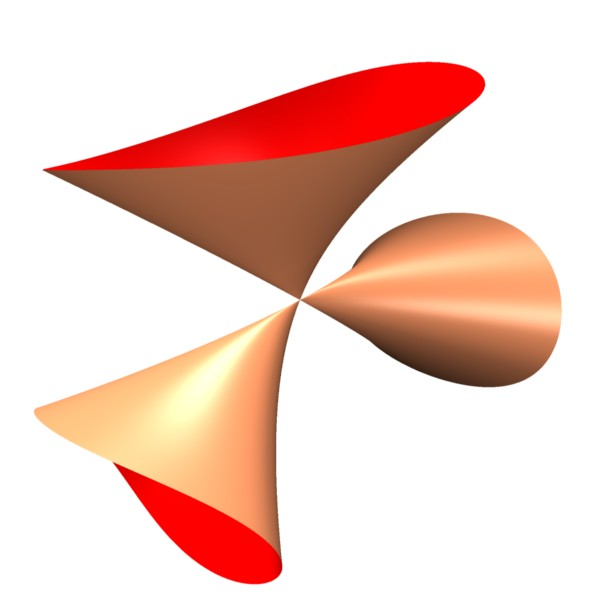
\includegraphics[width=1.2cm]{../../common/images/D4mm_0}\qquad%
		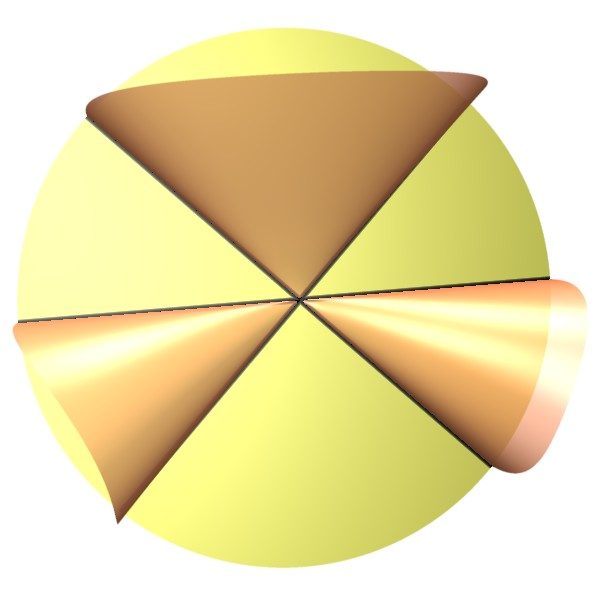
\includegraphics[width=1.2cm]{../../common/images/D4mm_def_with_plane_cut_0}%
	\end{Centering*}
	A good way to understand the geometry of this singularity is to look at the deformation
	\[
		(y+a)\cdot(x-y)\cdot(x+y)-z^2=0
	\]
	which splits it into three ordinary double points ($A_1$ singularities). Setting $a=0$ yields the original equation:
	\begin{Centering*}%
		\begin{tabular}{c@{\quad}c@{\quad}c}
			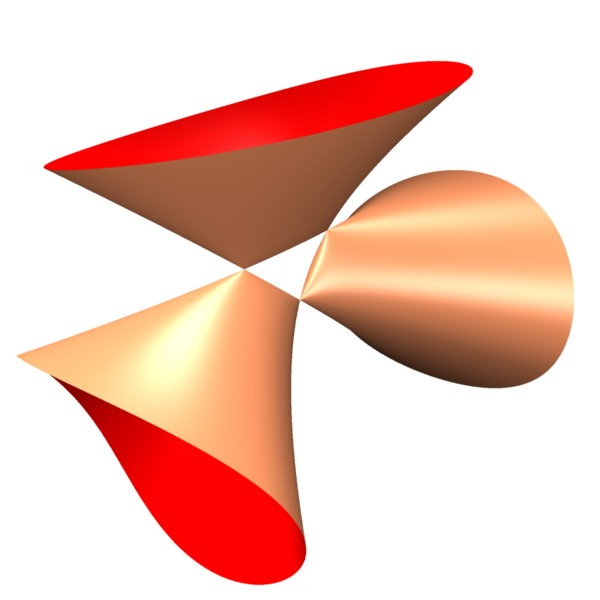
\includegraphics[width=1.2cm]{../../common/images/D4mm_1} &
			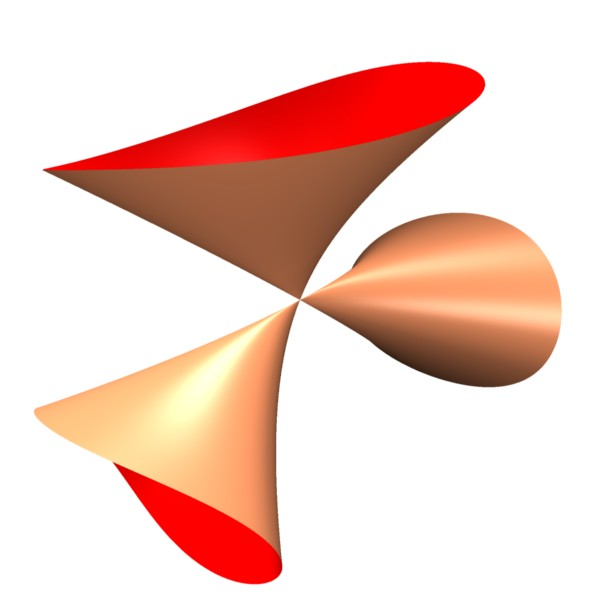
\includegraphics[width=1.2cm]{../../common/images/D4mm_0} &
			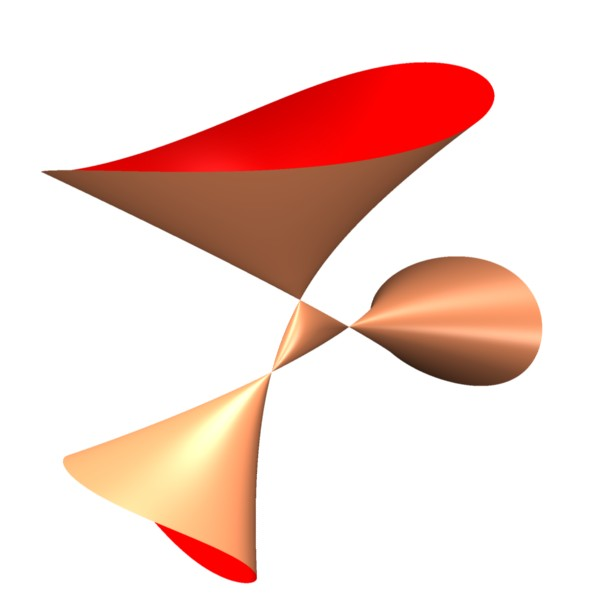
\includegraphics[width=1.2cm]{../../common/images/D4mm_2}\\
			$a=-0.5$ &
			$a=0$ &
			$a=0.5$
		\end{tabular}
	\end{Centering*}
\end{surferPage}
